\section{Styles}
%<-------------------------------------------------------------------------->
The look of a graph depends on three \TIKZ\ styles: \tkzname{VertexStyle},
\tkzname{EdgeStyle} and \tkzname{LabelStyle} (the labels of the edges).
There are several ways to change them; the last definition wins.

\begin{enumerate}
\item \tkzcname{GraphInit} chooses a predefined style (\tkzname{vstyle});
      \tkzcname{tkzDefGraphStyle} defines a new one.
\item \tkzcname{tkzSetUpGraph} changes the values used by the styles: colors,
      sizes, line widths\dots
\item The macros \tkzcname{SetVertexSimple}, \tkzcname{SetVertexNormal},
      \tkzcname{SetVertexShade}, \tkzcname{SetVertexArt},
      \tkzcname{SetUpVertex} and \tkzcname{SetUpEdge} refine a style.
\item The styles can be redefined with \tkzcname{tikzset}:
      \tkzname{VertexStyle/.style=\{\dots\}} defines a new style,
      \tkzname{VertexStyle/.append style=\{\dots\}} completes the current
      one.
\end{enumerate}

\subsection{\tkzcname{GraphInit}}
\begin{NewMacroBox}{GraphInit}{\oarg{local options}}
\begin{tabular}{llc}
\toprule
Options           & Default  & Definition \\
\midrule
\TOline{vstyle}   {Normal}   {predefined style}
\TOline{unit}     {\textbackslash GraphUnit}{unit of the graph}
\bottomrule
\end{tabular}

\medskip
\emph{The predefined styles are \tkzname{Empty}, \tkzname{Hasse},
\tkzname{Simple}, \tkzname{Classic}, \tkzname{Normal}, \tkzname{Shade},
\tkzname{Dijkstra}, \tkzname{Welsh}, \tkzname{Art} and \tkzname{Shade Art}.
The name of the style is not case sensitive. A style also sets the
behavior of the labels (inside, outside or no label).}
\end{NewMacroBox}

\subsubsection{The predefined styles}
\begin{center}
\def\tkzshowstyle#1{%
  \begin{tikzpicture}
    \GraphInit[vstyle=#1]
    \SetGraphUnit{1.6}
    \Vertex[Lpos=-90]{A}\EA[Lpos=-90](A){B}\Edge(A)(B)
  \end{tikzpicture}}
\begin{tabular}{*{5}{c}}
\tkzshowstyle{Empty}   & \tkzshowstyle{Hasse} & \tkzshowstyle{Simple} &
\tkzshowstyle{Classic} & \tkzshowstyle{Normal}\\
\tkzname{Empty} & \tkzname{Hasse} & \tkzname{Simple} &
\tkzname{Classic} & \tkzname{Normal}\\[6pt]
\tkzshowstyle{Shade}   & \tkzshowstyle{Dijkstra} & \tkzshowstyle{Welsh} &
\tkzshowstyle{Art}     & \tkzshowstyle{Shade Art}\\
\tkzname{Shade} & \tkzname{Dijkstra} & \tkzname{Welsh} &
\tkzname{Art} & \tkzname{Shade Art}\\
\end{tabular}
\end{center}

\begin{tkzexample}[latex=7cm,small]
\begin{tikzpicture}
  \GraphInit[vstyle=Dijkstra]
  \SetGraphUnit{3}
  \Vertex{A}\EA(A){B}
  \Edge[label=$7$](A)(B)
\end{tikzpicture}
\end{tkzexample}

\subsection{A new style: \tkzcname{tkzDefGraphStyle}}
\begin{NewMacroBox}{tkzDefGraphStyle}{\var{name}\var{code}}
\emph{Defines (or redefines) the style \tkzname{name} for
\tkzcname{GraphInit}\tkzname{[vstyle=name]}. The code is executed each time
the style is chosen; it can use the macros of this section or
\tkzcname{tikzset}. The name is not case sensitive.}
\end{NewMacroBox}

\begin{tkzexample}[latex=7cm,small]
\tkzDefGraphStyle{Red}{%
  \GraphInit[vstyle=Normal]
  \SetGraphColor{red!20}{red}}
\begin{tikzpicture}
  \GraphInit[vstyle=red]
  \Vertices[unit=1.5]{circle}{A,B,C,D}
  \Edges(A,B,C,D,A,C)
\end{tikzpicture}
\end{tkzexample}

\newpage
%<-------------------------------------------------------------------------->
\subsection{Settings: \tkzcname{tkzSetUpGraph}}
%<-------------------------------------------------------------------------->
The predefined styles use macros like \tkzcname{VertexShape} or
\tkzcname{EdgeLineWidth}. \tkzcname{tkzSetUpGraph} changes them with keys.

\begin{NewMacroBox}{tkzSetUpGraph}{\oarg{options}}
\begin{tabular}{lll}
\toprule
Options & Default  & Macro changed \\
\midrule
\TOline{vertex shape}      {circle}  {\textbackslash VertexShape}
\TOline{vertex line width} {0.5pt}   {\textbackslash VertexLineWidth}
\TOline{vertex line color} {black}   {\textbackslash VertexLineColor}
\TOline{vertex text color} {black}   {\textbackslash VertexTextColor}
\TOline{vertex fill}       {black}   {\textbackslash VertexFillColor}
\TOline{light fill}        {white}   {\textbackslash VertexLightFillColor}
\TOline{dark fill}         {black}   {\textbackslash VertexDarkFillColor}
\TOline{ball color}        {orange}  {\textbackslash VertexBallColor}
\TOline{inner sep}         {2pt}     {\textbackslash VertexInnerSep}
\TOline{outer sep}         {0pt}     {\textbackslash VertexOuterSep}
\TOline{small size}        {12pt}    {\textbackslash VertexSmallMinSize}
\TOline{medium size}       {18pt}    {\textbackslash VertexInterMinSize}
\TOline{big size}          {24pt}    {\textbackslash VertexBigMinSize}
\midrule
\TOline{edge color}        {black}   {\textbackslash EdgeColor}
\TOline{edge width}        {0.8pt}   {\textbackslash EdgeLineWidth}
\TOline{edge fill}         {orange}  {\textbackslash EdgeFillColor}
\TOline{art color}         {orange}  {\textbackslash EdgeArtColor}
\TOline{double distance}   {1pt}     {\textbackslash EdgeDoubleDistance}
\TOline{label text}        {black}   {\textbackslash LabelTextColor}
\TOline{label fill}        {white}   {\textbackslash LabelFillColor}
\midrule
\TOline{unit}              {1}       {\textbackslash GraphUnit}
\TOline{directed}          {}        {an arrow on every edge}
\TOline{arrow tip}         {stealth'}{tip of the arrows}
\bottomrule
\end{tabular}

\medskip
\emph{The changes are local: inside a \tkzname{tikzpicture} or a group they
stop at its end; in the preamble they apply to the whole document.
\tkzname{directed=false} cancels \tkzname{directed}, and the key \tkzname{-}
of \tkzcname{Edge} removes the arrow of one edge. The tips \tkzname{Stealth},
\tkzname{Latex}\dots\ need the library \tkzname{arrows.meta}, which is not
loaded by \tkzname{tkz-graph}.}
\end{NewMacroBox}

\begin{tkzexample}[latex=7cm,small]
\begin{tikzpicture}
  \tkzSetUpGraph[medium size=14pt,
     vertex line color=blue,
     light fill=blue!10,
     edge color=blue!60!black,
     edge width=1pt]
  \Vertices[unit=1.5,rotation=90]{circle}{A,B,C,D,E}
  \Edges(A,B,C,D,E,A)
\end{tikzpicture}
\end{tkzexample}

\begin{tkzexample}[latex=7cm,small]
% \usetikzlibrary{arrows.meta}
\begin{tikzpicture}
  \tkzSetUpGraph[directed,
    arrow tip={Stealth[length=6pt]}]
  \Vertices[unit=1.5,rotation=90,
            clockwise]{circle}{A,B,C,D,E}
  \Edges(A,B,C,D,E)
  \Edge[-](E)(A)
\end{tikzpicture}
\end{tkzexample}

\begin{tkzexample}[latex=7cm,small]
\begin{tikzpicture}
  \GraphInit[vstyle=Art]
  \tkzSetUpGraph[inner sep=8pt,
     edge width=3pt,ball color=blue!50]
  \Vertices[unit=2]{circle}{A,B,C,D,E}
  \Edges(A,B,C,D,E,A,C,E,B,D)
\end{tikzpicture}
\end{tkzexample}

\newpage
%<-------------------------------------------------------------------------->
\subsection{Refining a style}
%<-------------------------------------------------------------------------->
\begin{NewMacroBox}{SetVertexSimple}{\oarg{local options}}
\begin{tabular}{llc}
\toprule
Options   & Default  & Definition           \\
\midrule
\TOline{Shape}     {\textbackslash VertexShape}       {shape of the node}
\TOline{MinSize}   {\textbackslash VertexSmallMinSize}{minimum size}
\TOline{LineWidth} {\textbackslash VertexLineWidth}   {line width}
\TOline{LineColor} {\textbackslash VertexLineColor}   {color of the border}
\TOline{FillColor} {\textbackslash VertexFillColor}   {color of the inside}
\TOline{InnerSep}  {\textbackslash VertexInnerSep}    {inner sep}
\TOline{OuterSep}  {\textbackslash VertexOuterSep}    {outer sep}
\bottomrule
\end{tabular}

\medskip
\emph{Small filled vertices without label.}
\end{NewMacroBox}

\begin{tkzexample}[latex=7cm,small]
\begin{tikzpicture}
  \SetVertexSimple[Shape=diamond,
                   FillColor=blue!50]
  \Vertices[unit=2]{circle}{A,B,C,D,E}
  \Edges(A,B,C,D,E,A,C,E,B,D)
\end{tikzpicture}
\end{tkzexample}

\begin{NewMacroBox}{SetVertexNormal}{\oarg{local options}}
\begin{tabular}{llc}
\toprule
Options   & Default  & Definition           \\
\midrule
\TOline{Shape}     {\textbackslash VertexShape}         {shape of the node}
\TOline{MinSize}   {\textbackslash VertexInterMinSize}  {minimum size}
\TOline{LineWidth} {\textbackslash VertexLineWidth}     {line width}
\TOline{LineColor} {\textbackslash VertexLineColor}     {color of the border}
\TOline{FillColor} {\textbackslash VertexLightFillColor}{color of the inside}
\TOline{TextColor} {\textbackslash VertexTextColor}     {color of the label}
\TOline{InnerSep}  {\textbackslash VertexInnerSep}      {inner sep}
\TOline{OuterSep}  {\textbackslash VertexOuterSep}      {outer sep}
\bottomrule
\end{tabular}

\medskip
\emph{The labels are inside the vertices.}
\end{NewMacroBox}

\begin{tkzexample}[latex=7cm,small]
\begin{tikzpicture}
  \SetVertexNormal[Shape=rectangle,
                   LineWidth=2pt,
                   FillColor=green!50]
  \Vertices[unit=2]{circle}{A,B,C,D,E}
  \Edges(A,B,C,D,E,A,C,E,B,D)
\end{tikzpicture}
\end{tkzexample}

\begin{NewMacroBox}{SetVertexShade}{\oarg{local options}}
\emph{Options \tkzname{Shape}, \tkzname{MinSize}
(\tkzcname{VertexBigMinSize}), \tkzname{LineWidth}, \tkzname{LineColor},
\tkzname{BallColor} (\tkzcname{VertexBallColor}), \tkzname{InnerSep},
\tkzname{OuterSep}. Shaded vertices with their label; double edges.}
\end{NewMacroBox}

\begin{NewMacroBox}{SetVertexArt}{\oarg{local options}}
\emph{Same options as \tkzcname{SetVertexShade}, with
\tkzcname{VertexSmallMinSize} for \tkzname{MinSize}. Small shaded vertices
without label.}
\end{NewMacroBox}

\begin{tkzexample}[latex=7cm,small]
\begin{tikzpicture}
  \SetVertexShade[BallColor=red!60,
                  MinSize=20pt]
  \Vertices[unit=2]{circle}{A,B,C,D,E}
  \Edges(A,B,C,D,E,A)
\end{tikzpicture}
\end{tkzexample}

\newpage
\begin{NewMacroBox}{SetUpVertex}{\oarg{local options}}
\begin{tabular}{llc}
\toprule
Options         & Default  & Definition                       \\
\midrule
\TOline{Lpos}     {0}    {angle of an outside label}
\TOline{Ldist}    {0cm}  {distance of an outside label}
\TOline{Style}    {\{\}} {\TIKZ\ options added to the vertices}
\TOline{NoLabel}  {false}{no label}
\TOline{LabelOut} {false}{outside labels}
\TOline{Math}     {false}{labels in math mode}
\TOline{Unit}     {\textbackslash GraphUnit}{unit of the shortcuts}
\TOline{MinSize}  {\textbackslash VertexInterMinSize}{minimum size}
\TOline{LineWidth}{\textbackslash VertexLineWidth}{line width}
\TOline{LineColor}{\textbackslash VertexLineColor}{color of the border}
\TOline{FillColor}{\textbackslash VertexLightFillColor}{color of the inside}
\TOline{TextColor}{\textbackslash VertexTextColor}{color of the label}
\TOline{InnerSep} {\textbackslash VertexInnerSep}{inner sep}
\TOline{OuterSep} {\textbackslash VertexOuterSep}{outer sep}
\bottomrule
\end{tabular}

\medskip
\emph{Changes the current style of the vertices and the default values of
\tkzcname{Vertex}.}
\end{NewMacroBox}

\begin{tkzexample}[latex=7cm,small]
\begin{tikzpicture}
  \SetGraphUnit{3}
  \SetUpVertex[Lpos=-60,LabelOut,
               FillColor=yellow]
  \Vertex{A}\EA(A){B}\Edge(A)(B)
\end{tikzpicture}
\end{tkzexample}

\subsection{Colors of the predefined styles}
\begin{NewMacroBox}{SetGraphShadeColor}{\var{ball color}\var{edge color}\var{double color}}
\emph{Colors of the style \tkzname{Shade}.}
\end{NewMacroBox}

\begin{NewMacroBox}{SetGraphArtColor}{\var{ball color}\var{edge color}}
\emph{Colors of the style \tkzname{Art}.}
\end{NewMacroBox}

\begin{NewMacroBox}{SetGraphColor}{\var{fill color}\var{edge color}}
\emph{Colors of the style \tkzname{Normal}.}
\end{NewMacroBox}

\begin{tkzexample}[latex=7cm,small]
\begin{tikzpicture}
  \GraphInit[vstyle=Shade]
  \SetVertexNoLabel
  \SetGraphShadeColor{red!50}{black}{red}
  \Vertices[unit=2]{circle}{A,B,C,D,E}
  \Edges(A,B,C,D,E,A,C,E,B,D)
\end{tikzpicture}
\end{tkzexample}

\begin{tkzexample}[latex=7cm,small]
\begin{tikzpicture}
  \GraphInit[vstyle=Art]
  \SetGraphArtColor{green!40!black}{magenta}
  \Vertices[unit=2]{circle}{A,B,C,D,E}
  \Edges(A,B,C,D,E,A,C,E,B,D)
\end{tikzpicture}
\end{tkzexample}

\subsection{Other macros}
\begin{itemize}
\item \tkzcname{SetVertexLabeledSmall}, \tkzcname{SetVertexNotLabeledSmall}:
      small vertices with or without label and double edges;
\item \tkzcname{SetVertexForPresentation}\var{ball}\var{edge}\var{double}:
      style \tkzname{Shade} without label, with these colors;
\item \tkzcname{tkzSetUpColors}\tkzname{[background=\dots,text=\dots]}: the
      default colors of the background and of the text, used by the styles
      (this macro also changes the color of the page).
\end{itemize}

\subsection{Redefining \tkzname{VertexStyle} with \tkzcname{tikzset}}
\begin{tkzexample}[latex=7cm,small]
\begin{tikzpicture}
  \tikzset{VertexStyle/.style = {
      shape = circle, shading = ball,
      ball color = green!40!black,
      minimum size = 30pt, draw}}
  \SetVertexNoLabel
  \Vertex{A}\EA[unit=3](A){B}
  \Edge(A)(B)
\end{tikzpicture}
\end{tkzexample}

\endinput
